
This chapter presents results of the analysis of cancer data using the
software and algorithms presented in the previous chapter. In section
\ref{sec:analysis_tcgbiolinks} we present some use cases using mainly the TCGAbiolinks
package. In section \ref{sec:analysis_elmer} we present some data analysis using the ELMER package.
In section \ref{sec:glioma_analysis}, using the previous tools described we perfom a
glioma analysis focused specially in the two molecular subtypes G-CIMP-low and
 G-CIMP-high discovered by our laboratory and collaborators.

\section{Use cases using TCGAbiolinks}\label{sec:analysis_tcgbiolinks}

In this section, we introduce and describe the utility and application of TCGAbiolinks
through some use cases.
In subsection  \ref{subsec:analysis_tcgbiolinks2} we show a
lower-grade glioma downstream analysis with gene expression.
In subsection \ref{subsec:analysis_tcgbiolinks3} we show a
downstream analysis integration of gene expression and methylation data of colon
adenocarcinoma data, describing how to generate a starburst plot \cite{noushmehr2010identification},
which was introduced to illustrate the results of integrating
DNA methylation and gene expression data.


\subsection{Lower-grade glioma downstream analysis with gene expression} \label{subsec:analysis_tcgbiolinks2}

For this case study, we used the recently available \sigla{LGG}{lower-grade glioma} data to investigate gene expression differences between the reported molecular subtypes (IDHmutant, IDHwildtype and IDHmutant codels) \cite{platforms2015comprehensive}. In particular, we used TCGAbiolinks to download 293 samples profiled using messenger RNA expression (IlluminaHiSeq RNASeqV2) with available molecular subtypes. The data was normalized using the \textit{TCGAanalyze\_Normalization} function and we applied three filters to remove features/mRNAs with low signals across samples, obtaining 4578, 4284 and 1187 mRNAs, respectively. A clustering analysis was then applied using the ConsensusClusterPlus package \cite{wilkerson2010consensusclusterplus} which identified four distinct groups of samples (EC1-EC4) (Figure \ref{fig:caseexp}A). The survival curves for each cluster were generated using \textit{TCGAanalyze\_survival} and are shown in Figure \ref{fig:caseexp}B. As expected, each cluster effectively separated IDHwildtype tumors (EC1) from IDHmutant-non-codel (EC2) and IDHmutant-codel tumors (EC3 and EC4) (Figure \ref{fig:caseexp}). Additional biological subtypes (DNA methylation subtypes) were reproduced as expected (Figure \ref{fig:caseexp}D) \cite{platforms2015comprehensive}.

\begin{figure*}
\centering
%\includegraphics[width=.9\linewidth]{figures/case3_improved.pdf}
\includegraphics[width=1.0\linewidth]{images/figure4.pdf}
\caption[Case study - LGG downstream analysis with gene expression]{Case study - Integrative (or Downstream) analysis of gene expression and clinical data from LGG disease with unsupervised clustering and crossing expression clusters with clinical and molecular information. \textbf{(A)} Heatmap of 1187 more variables genes clustered with tree $k = 4$ in EC1, EC2, EC3, EC4. \textbf{(B)} Kaplan Meier survivals plot for EC clusters. \textbf{(C and D)} Distribution of the DNA Methylation clusters and ATRX mutation within the EC clusters.}
\label{fig:caseexp}
\end{figure*}

\subsection{Downstream analysis integration of gene expression and methylation data} \label{subsec:analysis_tcgbiolinks3}

The DNA methylation of specific promoter CpG islands has the potential to influence gene expression.
In this case study, we used TCGAbiolinks to examine the biological relationship between DNA methylation
and gene expression in \sigla{COAD}{Colon adenocarcinoma}. Using \textit{GDCquery}, \textit{GDCdownload}
and \textit{GDCprepare}, we obtained DNA methylation data (Infinium HumanMethylation450 and Infinium
HumanMethylation27 platforms) and gene expression data (IlluminaGA RNASeqV2 platform) for the same
TCGA COAD samples \cite{cancer2012comprehensive}. A supervised analysis was performed on the molecular
subtypes CIMP-Low [CIMP.L] and CIMP-High [CIMP.H].
The gene expression analysis started by the identification of outliers, followed by the normalization methods.
 Using \textit{TCGAanalyze\_DEA}, 34 DEGs ($log_2FC\geq 3.0$ and FDR $\leq 10^{-4}$) were identified.
 The result of this analysis is represented in a volcano plot (Figure \ref{fig:case_starburst}A)
 created using \textit{TCGAVisualize\_volcano}.
For the DNA methylation analysis,
using \textit{TCGAanlayze\_DMR} we identified 73 CpG-methylated probes ($\Delta\overline{\beta}\geq 0.25$ and  $FDR \leq 10^{-5}$;  (Figure \ref{fig:case_starburst}B). The DNA methylation and gene expression results were integrated as in the previous TCGA marker paper \cite{noushmehr2010identification,cancer2012comprehensive}, by generating a starburst plot (Figure \ref{fig:case_starburst}C) in which the x-axis is the $log_{10}$ of the correct P-value for DNA methylation and the y-axis is the $log_{10}$ of the correct P-value for the expression data.
The starburst plot highlights nine distinct quadrants.
To incorporate the DNA methylation difference cut-off into the  graph,
we highlighted genes that might have the potential for silencing due to epigenetic alterations.
 We highlighted five genes, EYA1, SIX2, ACSL6, OGDHL and SLC30A2, that showed a $\Delta\overline{\beta}\geq0.25$
 and a $log_2FC\geq 3.0$ between CIMP.L and CIMP.H.

\begin{figure*}
\centering
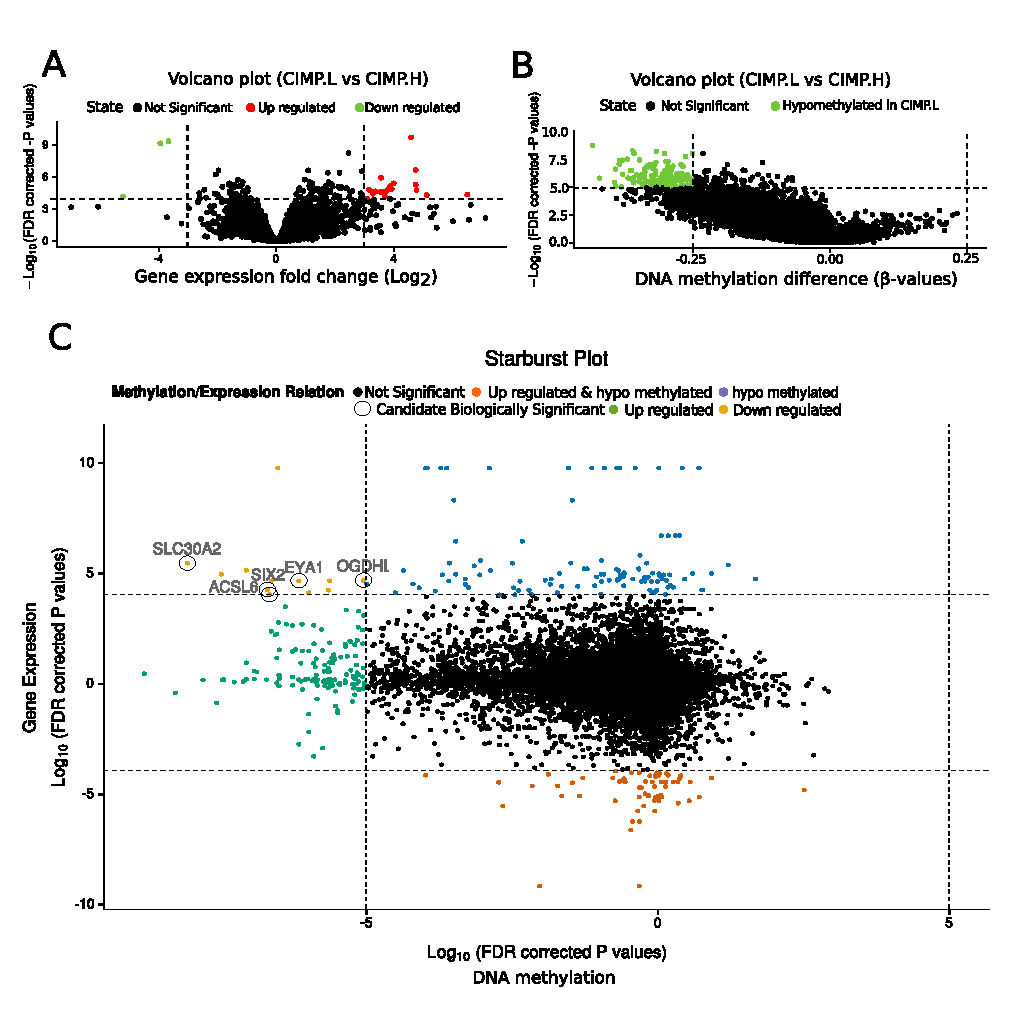
\includegraphics[width=1.0\linewidth]{images/figure5.pdf}
\caption[Case study - Integrative data analysis of Colon Adenocarcinoma]{
Case study - Integrative analysis of gene expression and DNA methylation data from COAD disease,
comparing groups CIMP.L and CIMP.H. \textbf{(A)} Expression volcano plot: fold change of expression data versus significance.
 \textbf{(B)} DNA methylation volcano plot: difference of DNA methylation versus significance.
 \textbf{(C)} Starburst plot: DNA methylation significance versus gene expression significance.}
\label{fig:case_starburst}
\end{figure*}


\section{Use cases using ELMER}\label{sec:analysis_elmer}

To exemplify the use of this new version we performed \textit{ELMER} analysis on TCGA BRCA (Breast Invasive Carcinoma) data retrieved directly from the GDC server by TCGAbiolinks. Use Case 1 compares tumor samples to normal samples using the \textit{Unsupervised} analysis mode, while Use Case 2 compares known BRCA molecular subtypes using the \textit{Supervised} mode. The HTML output report containing the code and results of both analysis are available as supplemental material and at \url{https://github.com/tiagochst/ELMER_supplemental/raw/master/supplemental_files.zip}.

%\newpage
\subsection{Use Case 1: Breast Invasive Carcinoma (Unsupervised mode)}

We performed \textit{ELMER} analysis comparing 778 Primary solid Tumor and 83 Solid Tissue Normal BRCA samples.  In this use case we wanted to be able to detect non pre-determined molecular subtypes among the tumor samples, so the percentage of samples used to identify the differentially methylated probes in function \textit{get.diff.meth}  was set to 20\% and the mode in function \textit{get.pair} and in function \textit{get.TFs} which was set to "unsupervised".
%In this mode we define the $U$ (unmethylated) group as the samples with lowest quintile of DNA methylation levels and the $M$ (methylated) group as the highest quintile.

This analysis showed that the set of differentially methylated CpG probes (DMCs) hypomethylated in the tumors and linked to the expression of a nearby gene had an enrichment for TFBS motifs for FOX family transcription factors (FOXA2, FOXA3, FOXA1, etc.) (Figure \ref{fig:motifplot}). For the most highly enriched motif FOAX3, the master regulator analysis identified \textit{FOXA1} as the top candidate among all TFs in the human genome (Figure \ref{fig:tfplot}), with the collaborating factors GATA3 and ESR1 as the next best candidates (Figure \ref{fig:scatter}). This illustrates the important point that \textit{in vitro} defined motifs from public TFBS databases are not always bound by the same TF family member \textit{in vivo}. This was the same result of the analysis in \citeauthor{yao2015inferring}, where we showed that ELMER identification of FOXA1, GATA3, and ESR1 were driven specifically by the ER+ (luminal A and luminal B) tumors. However, our unsupervised analysis (both in \citeauthor{yao2015inferring} and here) did not reveal Master Regulators for the other Breast Cancer molecular subtypes, such as Basal-like, HER2+, etc.

\begin{figure}
\centering
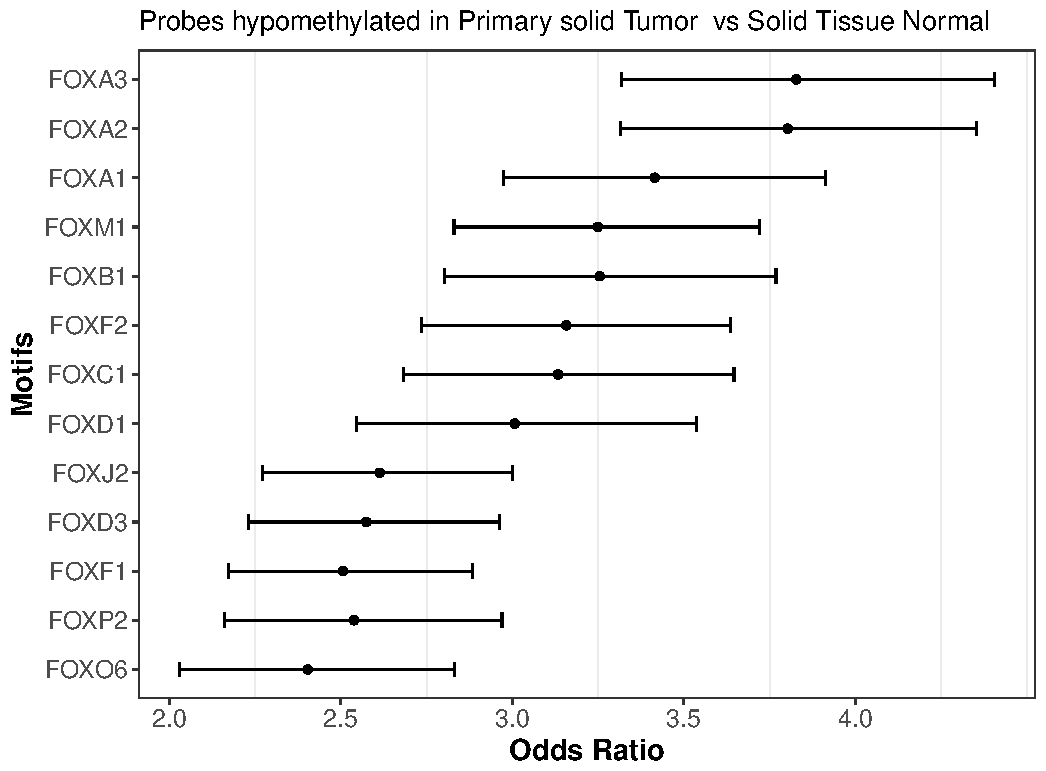
\includegraphics[width=1.0\textwidth]{images/motif_new.pdf}
\caption[Motif enrichment plot]{\label{fig:motifplot} Motif enrichment plot shows the enrichment levels ($OR\geq2.0$) for the most significant motifs based on the TCGA Breast Cancer Unsupervised analysis. A number of less significant motifs meet our default OR threshold of 1.1 ($\textit{lower.or}=1.1$), which can be browsed in our full Supplemental output report.}
\end{figure}

%\clearpage
\begin{figure}
\centering
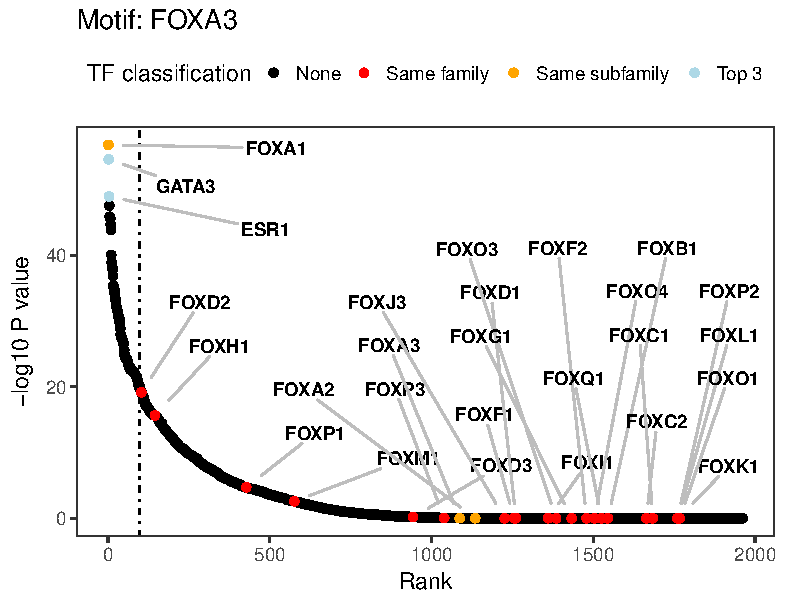
\includegraphics[width=0.9\textwidth]{images/TFranking.pdf}
\caption[TF ranking plot for FOXA3 motif]{\label{fig:tfplot} TF ranking plot shows the statistical $-log_{10}(P-value)$ assessing the anti-correlation level of candidate Master Regulator TF expression with average DNA methylation level for sites with the given motif (FOXA3). By default, the top 3 associated TFs (blue dots), and all of the TF family members (red dots) and subfamily members (orange dots) are labeled. The anti-correlation data for the top three candidates (FOXA1, GATA3, and ESR1) are derived from the data shown in Figure \ref{fig:scatter}}
\end{figure}

%\clearpage
\begin{figure}
\centering
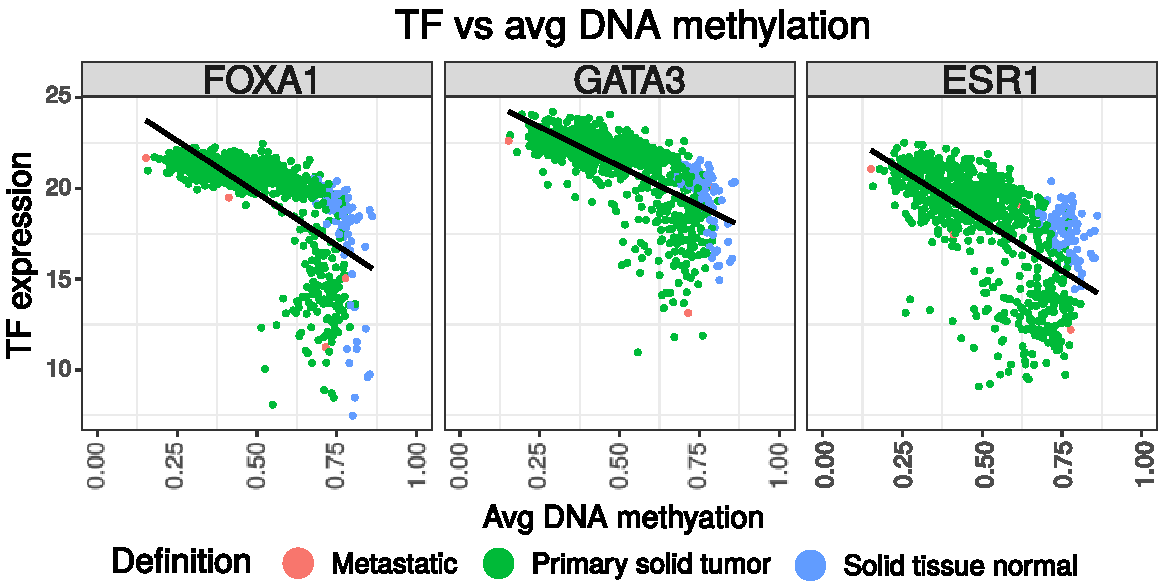
\includegraphics[width=1.0\textwidth]{images/scatter_font.pdf}
\caption[FOXA1, GATA3 and ESR1 expression vs average DNA methylation at probes with FOXA3 motif]{\label{fig:scatter} FOXA1, GATA3 and ESR1 were identified as the most significant Master Regulator candidates for the top motif (FOXA3). All FOX factors belonging to the same TFClass binding family are highlighted.}
\end{figure}


\subsubsection*{Functional annotation of cis-regulatory modules using \texttt{StateHub}}
While ELMER version 1 was limited to searching within annotated enhancer elements, we have since found that this constraint was not necessary to achieve statistical power. Thus ELMER 2.0 by default searches \textit{all} distal elements in the genome (distal elements are those greater than $\pm1 kb$ from a TSS; By changing ELMER default settings, it is possible to analyze TSS-proximal probes, either together with distal probes or separately.

Because ELMER can now search essentially all probes on the array, it is important to understand the context of the probes that result from an ELMER analysis. Typically these are enhancer probes, but some regulatory changes may involve promoters, insulators, etc. We used the \textit{StateHub} \cite{statepaintr} and \textit{FunciVar} Bioconductor packages, as described above, to characterize enrichment of the various cell-type-specific chromatin states in the significant BRCA-hypomethylated probes (Figure \ref{fig:funcivar}). Importantly, the MCF-7 cell line, and ER-positive breast cancer cell line, is much more strongly enriched for all enhancer and promoter classes than other cell types. As more reference cell types become available, this analysis will be useful in characterizing tumor GRN changes that reflect particular cell types or co-opted developmental programs.

%\afterpage{
\begin{figure}
\centering
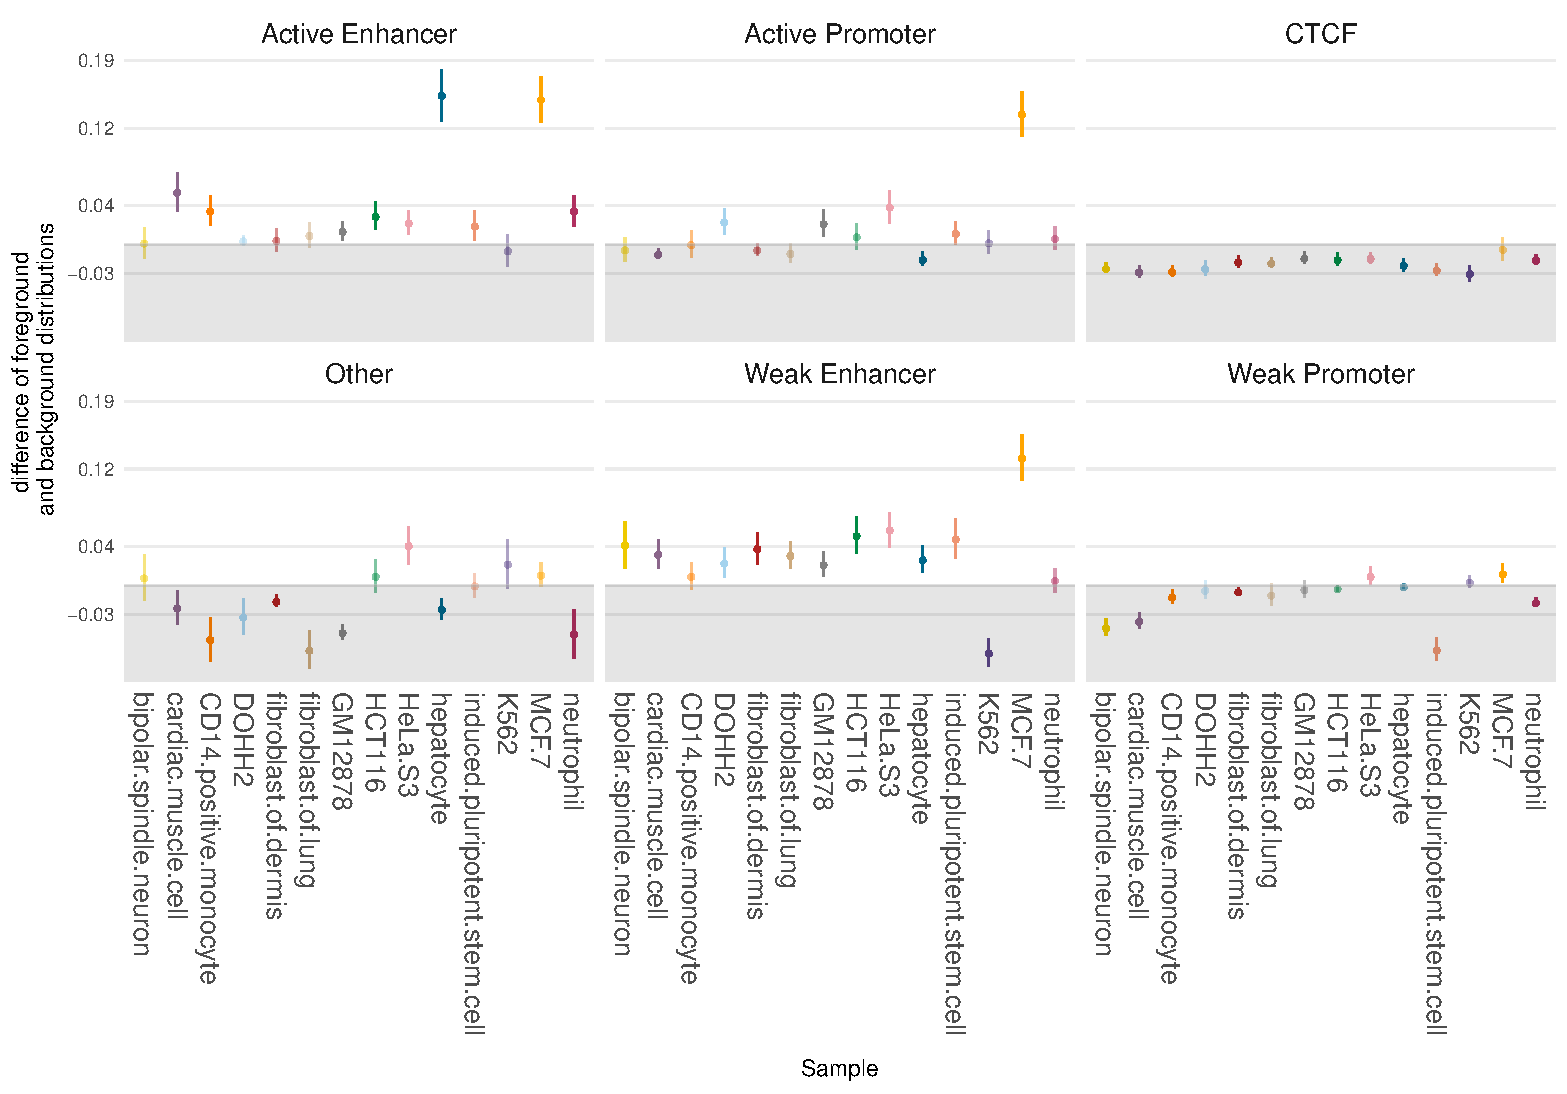
\includegraphics[width=0.8\textwidth]{images/funcivar.pdf}
\caption[Enrichment of paired probes and chromatin states of encode cells]{\label{fig:funcivar} Enrichment of paired probes and chromatin states of encode cells. The plot shows enrichment for enhancer active region, weak enhancer and active promoter region for MCF-7 cell. Acronyms - AR: Active region, EAR: active enhancer,
 EWR: Weak Enhancer, EPR: poised enhancer, PAR: active promoter, PWR: Weak Promoter,
 PPR: poised promoter, PPWR: Weak Poised Promoter, CTCF: architectural complex,
 TRS: transcribed, HET: heterochromatin, SCR: Polycomb Repressed Silenced. Y-axis shows the probability difference in overlap for the foreground class vs. random probes (Confidence Interval based on beta-binomial distribution.}
%\end{minipage}
\end{figure}
%}

%\clearpage


\subsubsection*{Comparing inferred results with MCF-7 chIA-PET}

As shown in \citeonline{yao2015inferring}, we compared the putative pairs inferred to the chromatin loops derived from deep-sequenced ChIA-PET data from ER+ Breast Cancer MCF7 cells \cite{li2012extensive}. First, we identify the number of \textit{ELMER} pairs overlapping the ChIA-PET loops, then we repeat using randomly generated  pairs with properties similar to the \textit{ELMER} pairs. For each true ELMER probe in a probe-gene pair, we randomly select a different probe from the complete set of distal probes. We then choose the nth nearest gene to the random probe, where n is the same as the adjacency of the true ELMER probe (i.e. if the true probe is linked to the second gene upstream, the  random probe will also be linked to its second gene upstream). Thus, the random linkage set has both the same number of probes and the same number of linked genes as the true set. One hundred such random datasets were generated to arrive at a 95\% CI ($\pm 1.96* SD$).
The result is shown in Figure \ref{fig:chiapet}. ELMER pairs were enriched for ChIA-PET loops by roughly 3-fold over random pairs.



\begin{figure}
\centering
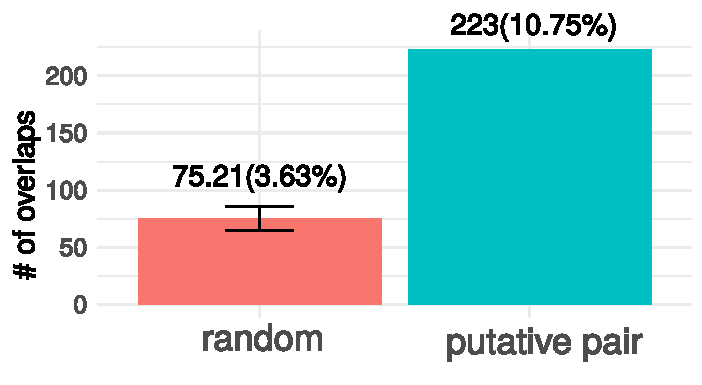
\includegraphics[width=0.5\textwidth]{images/mcf7.pdf}
\caption[MCF7 ChIA-PET validation]{\label{fig:chiapet} The graph shows the comparison of the number of probe-gene pairs identified within MCF7 ChIA-PET data using the putative pairs from BRCA vs. random pairs}
\end{figure}

%\clearpage
\subsection{Use Case 2: BRCA molecular subtypes analysis (Supervised mode)}


Several studies identified distinct molecular Breast Cancer molecular subtypes including luminal-like (Luminal A and Luminal B) subclasses, which are Estrogen receptor-positive (ER-positive), and the basal-like, ErbB2-positive and normal-like subclasses (ER-negative) \cite{perou2000molecular,yersal2014biological,sorlie2001gene}. We performed \textit{ELMER} analysis comparing known molecular subtypes (Her2, Luminal A, Luminal B and Basal-like) using the TCGA BRCA dataset and classifications retrieved from \cite{ciriello2015comprehensive} using TCGABiolinks.
% TIAGO IS THIS CORRECT?  DID YOU USE BIOLINKS?
% Yes, the data was downloaded using TCGAbiolionks
% The annotation was added manually

We performed pairwise analyses between different molecular subtypes. It is important to note that we expect these analyses to have increased statistical power over Unsupervised analyses, as illustrated above in Figure \ref{fig:mode}. One useful output plot is the comprehensive heatmap,
which illustrates the identification of inverse correlated probe-gene pairs (Figure \ref{fig:heatmap}) for the LumA vs Basal-like analysis.

\begin{figure}[ht!]
\centering
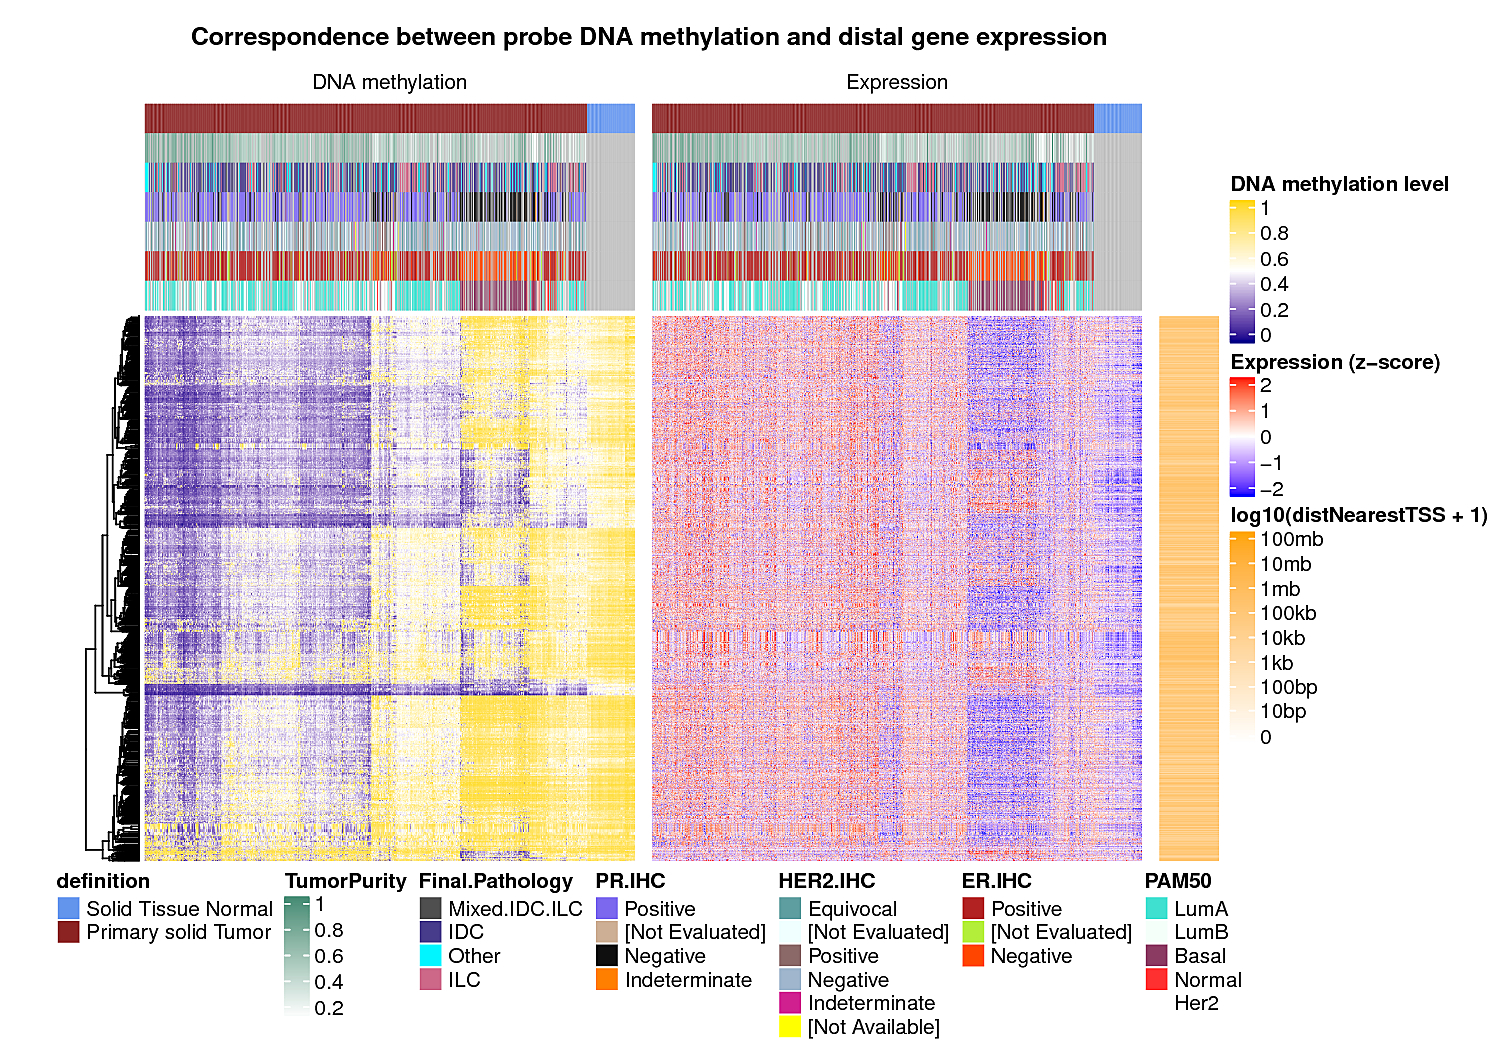
\includegraphics[width=1.0\textwidth]{images/heatmap.jpg}
\caption[Heatmap of inverse correlated probe and gene pairs ]{\label{fig:heatmap} The comprehensive heatmap view shows all probe / gene pairs identified by ELMER, clustered according to similarity. This plot is based on the Supervised analysis of LumA vs Basal-like Breast Cancer cases. The inverse correlation between methylation and expression can be observed.}
\end{figure}

The unsupervised analysis of the same sample identified several Luminal type Master Regulators (MRs) such as FOXA1, GATA3, and ESR1. In order to identify MRs for the other subtypes, we created a table  (Table \ref{tbl:TF_molecular}) of candidate MRs identified by each pairwise ELMER run (complete results can be found in the supplemental HTML file described in the Supplementary Methods section).

Interestingly, several new MRs are identified for the Basal-like group, and these were mostly consistent in comparisons against Luminal and HER2+ subtypes. One group of MRs identified are the \textit{SOX10} and \textit{SOX9} TF signatures. For these signatures, the regulatory TF candidate identified are the \textit{SOX9} (Sry-related HMG box-9) TF and \textit{SOX11} (Sry-related HMG box-11) TF; this correlation between basal-like and SOX11 was recently described by \cite{shepherd2016sox11} and \textit{SOX9} was described by \cite{gong2015foxa1}. Most interestingly, we found KLF5 to be a consistently predicted MR for the Basal-like breast subtype. KLF5 is a master pluripotency factor of embryonic stem cells, and has been associated with a number of different cancers. In breast cancer, it's overexpression has been linked to aggressive, ER-negative and basal-like breast cancers \cite{ben2008embryonic}. % PUBMED ID 18443585

\begin{table}[]
\centering
{\small
\caption[BRCA supervised analysis: Candidate master regulator TFs (MRs) for each molecular subtype found in a pairwise comparison]{Use case 2 - BRCA supervised analysis: Candidate master regulator TFs (MRs) for each molecular subtype found in a pairwise comparison. This table only includes MRs occurring in multiple pairwise comparisons.}
\label{tbl:TF_molecular}
\begin{tabular}{@{}|c|c|c|c|c|c|c|c|c|@{}}
\midrule
\textit{\textbf{TF}} & \textbf{\begin{tabular}[c]{@{}c@{}}LUMA \\ (vs basal)\end{tabular}} & \textbf{\begin{tabular}[c]{@{}c@{}}LUMB \\ (vs basal)\end{tabular}} & \textbf{\begin{tabular}[c]{@{}c@{}}Basal \\ (vs LumB)\end{tabular}} & \textbf{\begin{tabular}[c]{@{}c@{}}Basal \\ (vs HER2)\end{tabular}} & \textbf{\begin{tabular}[c]{@{}c@{}}HER2 \\ (vs Basal)\end{tabular}} \\ \midrule
\textit{\textbf{AR}} & x & x &  &  &  \\
\textit{\textbf{BCL11A}} &  &  & x & x &  \\
\textit{\textbf{CEBPB}} &  &  & x & x &  \\
\textit{\textbf{E2F3}} &  &  & x & x &  \\
\textit{\textbf{EMX1}} & x & x &  &  &  \\
\textit{\textbf{ESR1}} & x & x &  &  &  \\
\textit{\textbf{ETV6}} &  &  & x & x &  \\
\textit{\textbf{FOXA1}} & x & x &  &  & x \\
\textit{\textbf{FOXP1}} & x & x &  &  & x \\
\textit{\textbf{GATA3}} & x & x &  &  & x \\
\textit{\textbf{GLI1}} & x & x &  &  &  \\
\textit{\textbf{HOXB1}} & x & x &  &  &  \\
%\textit{\textbf{HOXB2}} & x & x &  &  & x \\
\textit{\textbf{HOXB3}} &  &  &  &  & x \\
%\textit{\textbf{HOXB6}} &  &  &  &  & x \\
\textit{\textbf{HOXC10}} &  &  &  &  & x \\
%\textit{\textbf{HOXC11}} &  &  &  &  & x \\
\textit{\textbf{KLF5}} &  &  & x & x &  \\
\textit{\textbf{LMX1B}} & x & x &  &  &  \\
\textit{\textbf{NR2E3}} & x & x &  &  &  \\
%\textit{\textbf{PATZ1}} &  & x &  &  &  \\
\textit{\textbf{PBX1}} &  & x &  &  &  \\
\textit{\textbf{RARA}} & x & x &  &  &  \\
%\textit{\textbf{RUNX3}} &  &  & x &  &  \\
\textit{\textbf{SOX8}} &  &  & x & x &  \\
\textit{\textbf{SOX9}} &  &  & x & x &  \\
\textit{\textbf{SOX11}} &  &  & x &  &  \\
\textit{\textbf{ZNF467}} & x & x &  &  &  \\
\textit{\textbf{ZIC1}} &  &  & x & x &  \\  \hline
\end{tabular}
}
\end{table}
